Given a model transformation $\MT\colon \Lang(C^S) \TransMT \Lang(D_2)$ from source DSL $\Lang(C^S)$ that is restricted by source domain graph constraints $C^S$ to target DSL $\Lang(D_2)$ in target domain $D_2$, then $\MT$ is domain complete if each source model $G^S \in \Lang(C^S)$ can be completely translated via a model transformation sequence in the sense that all elements of the graph are translated exactly once by changing their translation attributes from $\False$ to $\True$.

\paragraph*{General Assumption:}
As with the results for verifying domain completeness in \cref{sec-dc-verification}, we assume that the results of this Chapter are applied in the context $(\ATrGraphs_\ATGI,\M)$ of typed, attributed triple graphs with node type inheritance and common triple type graph $\ATGI$.
This is due to the fact that the node and edge attributes are used as markings (translation attributes) for checking conflict-freeness of rules.
Moreover, translation attributes are used for an intuitive definition of domain completeness of model transformations in \cref{def:sec-dom-compl-met:dc}.
Note that according to \cref{sec-dc-general,def:sec-dc-general:lang}, we write $C$ short for a set of constraints $C=C_I \cup C_G$ that is composed of constraints $C_I$ that are designated for initial satisfaction and constraints $C_G$ that are designated for general satisfaction.
Analogously, we write $\Lang(C)$ short for $\Lang_I(C_I) \cap \Lang(C_G)$.
%If not made explicit, we assume that a given triple graph grammar $\TGG$ and domain constraints $C$ are typed over the same type graph.

\begin{definition}[Domain Completeness of Model Transformations]
\label{def:sec-dom-compl-met:dc}
Let $C^S$ be the set of source domain graph constraints and $\Lang(C^S)$ be the source domain-specific language of graphs. 
Furthermore, let $\TGG$ be a triple graph grammar that specifies the translation $\MT\colon \Lang(C^S) \TransMT \Lang(D_2)$ of graphs in $\Lang(C^S)$ into graphs in the target domain-specific language $\Lang(D_2)$.
%For typing, $C^S$ is typed over some type graph $\TG^S$ and $\TGG$ is typed over some triple type graph $(\TG^S \gets \TG^C \to \TG^T)$, i.e., both coincide on $\TG^S$.
\emph{The model transformation $\MT$ is domain complete}\index{model transformation!domain completeness}, if for each graph $G^S \in \Lang(C^S)$ there is a model transformation sequence $(G^S,G_0 \Trans{\tr^*_\FT} G_n,G^T)$ based on the forward translation rules of $\TGG$ with $G_0=(\Att^\False(G^S) \gets \varnothing \to \varnothing)$ and $G_n=(\Att^\True(G^S) \gets G^C \to G^T)$.
\envEndMarker
\end{definition}

Based on the ``classical" syntactical completeness and correctness of model transformations by TGGs based on forward translation rules (cf. \cref{sec-gen-intro-compl,rem:sec-gen-intro-compl:classical_corr_compl_mt}), the domain completeness of model transformations from \cref{def:sec-dom-compl-met:dc} can be redefined as follows.
While \cref{def:sec-dom-compl-met:dc} reflects the intuitive meaning behind complete transformations, \cref{fact:sec-dom-compl-mt:comp} expresses completeness in terms of a language inclusion which can be verified by using the verification techniques for domain completeness.
Therefore, both formulations of completeness in \cref{def:sec-dom-compl-met:dc,fact:sec-dom-compl-mt:comp} are equivalent.

\begin{theorem}[Domain Completeness of Model Transformations]
\label{fact:sec-dom-compl-mt:comp}
Let $\MT\colon \Lang(C^S) \TransMT \Lang(D_2)$ be a model transformation based on forward translation rules of a given $\TGG$.
Transformation $\MT$ is domain complete according to \cref{def:sec-dom-compl-met:dc} if and only if domain completeness w.r.t. $\Lang(C^S)$ and $\Lang(\TGG)^S$ holds in the sense of \cref{sec-dc-general,def:sec-dc-general:dcp}, i.e., $\Lang(C^S) \subseteq \Lang(\TGG)^S$.
\envEndMarker
\end{theorem}

\begin{proof}
\begin{enumerate}
  \item[\textbf{``$\Rightarrow$''}] For each $G^S \in \Lang(C^S)$ with corresponding model transformation sequence based on forward translation rules the ``classical" correctness implies that $G^S \in \Lang(\TGG)^S$ (cf. \cref{sec-gen-intro-compl,rem:sec-gen-intro-compl:classical_corr_compl_mt}).
  \item[\textbf{``$\Leftarrow$''}] By ``classical" completeness, for each $G^S \in \Lang(C^S) \cap \Lang(\TGG)^S$ there is a model transformation sequence $(G^S,G_0 \Trans{\tr^*_\FT} G_n,G^T)$ based on forward translation rules with $G_0=(\Att^\False(G^S) \gets \varnothing \to \varnothing)$ and $G_n=(\Att^\True(G^S) \gets G^C \to G^T)$ (cf. \cref{sec-gen-intro-compl,rem:sec-gen-intro-compl:classical_corr_compl_mt}).
\end{enumerate}
\end{proof}

%For TGGs without application conditions, 
Similarly to the verification of domain completeness for flat graphs in \cref{sec-dc-verification,thm:C-extensionCompleteness}, we verify the language inclusion $\Lang(C^S) \subseteq \Lang(\TGG)^S$ by verifying $C^S$-conflict-freeness from \cref{thm:C-extensionCompleteness} w.r.t. forward translation rules $\TR_\FT$, since, we only need to check for possible overlappings of extensions in the source domain.
Therefore, similarly to \cref{sec-dc-verification,def:cf-marking-rules}, we define the $C^S$-conflict-freeness of forward translation rules in \cref{def:sec-dom-compl-mt:cf-fwd}.
Note that in $C^S$-conflict-freeness of forward translation rules, only critical pairs need to be considered where the source component of the conflict triple graph $O$ occurs in graphs of $\Lang(C^S)$ (cf. \cref{def:sec-dom-compl-mt:cf-fwd,def:sec-dom-compl-mt:cf-fwd:1}) and conflict triple graph $O$ can be embedded in a triple graph $O'$ that can be created by a forward translation sequence (cf. \cref{def:sec-dom-compl-mt:cf-fwd,def:sec-dom-compl-mt:cf-fwd:2}).

\begin{definition}[$C^S$-Conflict-Freeness of Forward Translation Rules]
\label{def:sec-dom-compl-mt:cf-fwd}
Let $C^S$ be the source domain constraints and $\TR_\FT$ be the forward translation rules of triple rules $\TR$.
Then, \emph{$\TR_\FT$ is $C^S$-conflict-free}\index{triple rule!forward translation rule!$C$-conflict-freeness}, if for each critical pair $(K_1 \TransB{(\tr_{\FT,1},o_1)}\nobreak O=(O^S \gets O^C \to O^T) \Trans{(\tr_{\FT,2},o_2)} K_2)$ with $\tr_{\FT,1},\tr_{\FT,2} \in \TR_\FT$ where 
\begin{enumerate}
  \item \label{def:sec-dom-compl-mt:cf-fwd:1}$O^S$ is significant w.r.t. $\Lang(C^S)$ (or not $C^S$-inconsistent), and
  \item \label{def:sec-dom-compl-mt:cf-fwd:2}there is $O \to O' \in \M$ and forward translation sequence $(\Att^\False(\ol{O}) \gets \varnothing \to \varnothing) \Trans{\tr_\FT^*} O'$ via $\TR_\FT$,
\end{enumerate}
it is true that the rules and matches are the same ($\tr_{\FT,1}=\tr_{\FT,2},o_1=o_2$) (or it is true that the critical pair is strictly confluent).
\envEndMarker
\end{definition}

\begin{theorem}[Domain Completeness of Model Transformations]
% without Application Conditions]
\label{thm:sec-dom-compl-mt-without-acs}
Let $C^S$ be the source domain constraints in $\M$-normal form, $\Lang(C^S)$ be the source domain-specific language over $C^S$ and $\Lang(\TGG)$ be the language over a non-deleting triple graph grammar $\TGG=(\varnothing,\TR)$ with empty triple start graph $\varnothing$, all triple productions $\TR$ being non-trivial and where all application conditions are in $\M$-normal form.
Let $\TR_\FT$ be the derived set of forward translation rules from $\TGG$.
Furthermore, let $\MT$ be a model transformation based on forward translation rules $\TR_\FT$.
If the rules $\TR_\FT$ are $C^S$-conflict-free and $\Lang(\TGG')^S$ is $C^S$-extension complete where $\TGG'=(\varnothing',\TR)$ with $\varnothing'$ being the empty triple start graph with $\DSIG$-term algebra $T_\DSIG(X)$, then domain completeness w.r.t. $\Lang(C^S)$ and $\Lang(\TGG)^S$ holds for almost injective matches, i.e., it holds that $\Lang(C^S) \subseteq \Lang(\TGG)^S$.
\envEndMarker
\end{theorem}

\begin{proof}
The proof is basically identical to the proof of \cref{thm:C-extensionCompleteness}.
Let $G \in \Lang(C^S)$, $i\colon G_A \to G$ be an instance morphism and $A=(a_i)_{i \in \{1,\ldots,n\}} \in Atoms(G_A)$ be the atoms of $G_A$.
Analogously to \cref{thm:C-extensionCompleteness}, by $\forall a \in A.a \in EAtoms(C^S)$ and $\Lang(\TGG')^S$ is $C^S$-extension complete it follows that $\forall a \in A.\exists S_a \in Extensions(a,C^S_G)$ such that $S_a \subseteq \Lang(\TGG')^S$ by \cref{def:C-extensionCompleteness}.
Thus, $\forall a \in A.\exists S_a \in Extensions(a,C^S_G)$ such that $\forall s \in S_a.\exists$ triple graph $(s \gets s^C \to s^T) \in \Lang(\TGG')$ and model transformation sequence $(s,(\Att^\False(s) \gets \varnothing \to \varnothing) \Trans{\tr_\FT^*} (\Att^\True(s) \gets s^C \to s^T),s^T)$ based on forward translation rules $\TR_\FT$ by model transformation $\MT$ and \cref{sec-gen-intro-compl,rem:sec-gen-intro-compl:classical_corr_compl_mt}.
Note that for each such model transformation sequence and a given injective embedding $f\colon s \to s' \in \M$ there is a forward translation sequence $(\Att^\False(s') \gets \varnothing \to \varnothing) \Trans{\tr_\FT^*} (s' \oplus \Att^\True_{s} \oplus \Att^\False_{s' \setminus s} \gets s^C \to s^T)$ via forward translation rules $\TR_\FT$ analogously to \cref{sec-dc-verification,lem:equivalence-marking-emptySG} $^{(*^A)}$, since, all relevant elements of application conditions in rules $\TR_\FT$ are marked with $\True$ whereas the marking of all elements in $s' \setminus s$ remain $\False$ for the translation sequence and therefore, cannot be matched by the application conditions.
Analogously to the proof of \cref{thm:C-extensionCompleteness}, there is a function $f_{a_E}$ with $f_{a_E}(a)=s \in S_a,\forall a \in A=(a_i)_{i \in \{1,\ldots,n\}}$ such that there exist graphs $(G^E_j)_{1 \leq j \leq n-1}$ and pushouts $(PO^E_k +_{G^E_k} f_{a_E}(a_{k+1})=PO^E_{k+1})_{k \in \{1,\ldots,n-1\}}$ with pushout objects $PO^E_{k+1}$, $PO^E_1=f_{a_E}(a_1)$ and injective embeddings $i_{k,1}\colon PO^E_k \to PO^E_{k+1}$ and $i_{k,2}\colon f_{a_E}(a_{k+1}) \to PO^E_{k+1} \in \M$ where $PO^E_n=G_A$ by \cref{sec-dc-verification,lem:union-ext-atoms}.
For pushout $k=1$ we conclude as follows.
By $(*^A)$, there exists forward translation sequences $t_1\colon (\Att^\False(PO^E_2) \gets \varnothing \to \varnothing) \Trans{\tr_\FT^*} (PO^E_2 \oplus \Att^\True_{f_{a_E}(a_1)} \oplus \Att^\False_{PO^E_2 \setminus f_{a_E}(a_1)} \gets f_{a_E}(a_1)^C \to f_{a_E}(a_1)^T)$ and $t_2\colon (\Att^\False(PO^E_2) \gets \varnothing \to \varnothing) \Trans{\tr_\FT^*} (PO^E_2 \oplus \Att^\True_{f_{a_E}(a_2)} \oplus \Att^\False_{PO^E_2 \setminus f_{a_E}(a_2)} \gets f_{a_E}(a_2)^C \to f_{a_E}(a_2)^T)$ via forward translation rules $\TR_\FT$.
Analogously to the proof of \cref{thm:C-extensionCompleteness}, assumption $\TR_\FT$ is $C^S$-conflict-free implies that transformation system $\TR_\FT$ is confluent and therefore, there is a complete forward translation sequence $(\Att^\False(PO^E_2) \gets \varnothing \to \varnothing) \Trans{\tr_\FT^*} (\Att^\True(PO^E_2) \gets C_2 \to T_2)$, i.e., a model transformation sequence $(PO^E_2,(\Att^\False(PO^E_2) \gets \varnothing \to \varnothing) \Trans{\tr_\FT^*} (\Att^\True(PO^E_2) \gets C_2 \to T_2),T_2)$ based on forward translation rules $\TR_\FT$ for pushout object $PO^E_2$.
Note that the restriction to a subset of all critical pairs in $C^S$-conflict-freeness matches the situation, since, $G^A \in \Lang(C^S)$ and $\M$-composition of embeddings $i_{k,1},i_{k,2}$ imply that the source component of all conflict triple graphs of conflicts that may occur is significant w.r.t. $\Lang(C^S)$ (cf. \cref{def:sec-dom-compl-mt:cf-fwd,def:sec-dom-compl-mt:cf-fwd:1}) and furthermore, all such conflict triple graphs of conflicts that may occur are embedded in triple graphs that are created by forward translation sequences $t_1$ and $t_2$ (cf. \cref{def:sec-dom-compl-mt:cf-fwd,def:sec-dom-compl-mt:cf-fwd:2}).
Analogously, we iterate over all pushouts for $k=(1,\ldots,n-1)$ and obtain a model transformation sequence $(PO^E_n,(\Att^\False(PO^E_n) \gets \varnothing \to \varnothing) \Trans{\tr_\FT^*} (\Att^\True(PO^E_n) \gets C_n \to T_n),T_n)$ based on forward translation rules $\TR_\FT$ and almost injective matches.
By \cref{sec-gen-intro-compl,rem:sec-gen-intro-compl:classical_corr_compl_mt}, $PO^E_n=G_A \in \Lang(\TGG')^S$, i.e., there is $\varnothing' \Trans{*} (G_A \gets C_A \to T_A)$ via $\TR$.
We extend instance morphism $i\colon G_A \to G$ to a triple graph morphism $i'\colon (G_A \gets C_A \to T_A) \to (G \gets C \to T)$ that is an instance morphism componentwise for source, correspondence and target.
Analogously to the proof of \cref{thm:C-extensionCompleteness} by \cref{lem:atiti} componentwise with instance morphism $i'$ and all application conditions in $\TR$ being in $\M$-normal form there is a transformation $\varnothing \Trans{*} (G \gets C \to T)$ via $\TR$ and almost injective matches, i.e., $G \in \Lang(\TGG)^S$.
Therefore, $\Lang(C^S) \subseteq \Lang(\TGG)^S$.
\end{proof}

% For TGGs with application conditions, we additinal have to check for conflicts with application conditions in the target domain.
% Therefore, we use consistency creating rules instead of forward translation rules and omit critical pairs that overlap in the correspondence or target part.
% 
% \begin{definition}[C-conflict-freeness of Consistency Creating Rules]
% \label{def:cf-marking-rules}
% Let $C^S$ be a set of source domain constraints and let $\TR_\CC$ be the set of consistency creating rules as derived from a given $\TGG$.
% Then, \emph{$\TR_\CC$ is $C^S$-conflict-free}\index{consistency creating rule!C-conflict-freeness}, if for each critical pair $K_1 \TransB{p_1,o_1}\nobreak O \Trans{p_2,o_2} K_2$ that does not overlap in the correspondence and target part and is not $C^S$-inconsistent with $p_1,p_2 \in \TR_\CC$ it is true that the rules and matches are the same ($p_1=p_2,o_1=o_2$).
% \envEndMarker
% \end{definition}
% 
% \begin{theorem}[Domain Completeness of Model Transformations with Application Conditions]
% \label{thm:sec-dom-compl-mt-with-acs}
% Let $C^S$ be the source domain constraints, $\Lang(C^S)$ be the source domain language and $\Lang(\TGG)$ be the language over a non-deleting $\TGG$ with empty start triple graph.
% Let $\TR_\CC$ be the derived set of consistency creating rules from $\TGG$.
% If the rules $\TR_\CC$ are $C^S$-conflict-free and $\Lang(\TGG)^S$ is $C^S$-extension complete, then domain completeness w.r.t. $\Lang(C^S)$ and $\Lang(\TGG)^S$ holds, i.e., $\Lang(C^S) \subseteq \Lang(\TGG)^S$.
% \envEndMarker
% \end{theorem}
% 
% \nn{
% \begin{proof}
% 
% \end{proof}
% }

According to domain completeness under restrictions in \cref{sec-dc-general-res}, we define domain completeness of model transformations under restrictions.
This is important for model transformations that only cover specific elements of each graph in the source DSL.
For example, the model transformation in \cref{sec-dc-general-res} from class diagrams (CDs) to relational database models (RDBMs) only covers the elements of the restricted type graph $\TG_{\CD,R}$ in \cref{fig:sec-dc-general:res_tg}, i.e., classes and their attributes in class diagrams, while neglecting class constructors and their visibilities.
In contrast to ``full'' domain completeness of the transformation which requires that all class diagrams can be completely translated into RDBMs, domain completeness under restrictions only requires that all classes and their attributes in each class diagram can be completely translated into corresponding tables and columns.

\begin{definition}[Domain Completeness of Model Transformations under Restrictions]
\label{def:sec-dom-compl-mt:dom_compl_res_mt}
Let $t\colon \TG^S_R \to \TG^S \in \M$ be a type morphism and $\TG^S_R$ be the restriction of source type graph $\TG^S$.
Let $\TG=(\TG^S_R \gets \TG^C \to \TG^T)$ be a triple type graph.
Let $C^S$ be the set of source domain graph constraints typed over $\TG^S$ and $\Lang(C^S)$ be the source domain-specific language of graphs. 
Furthermore, let $\TGG$ be a triple graph grammar typed over $\TG$ that specifies the translation $\MT\colon \Lang(C^S) \TransMT \Lang(D_2)$ of graphs in $\Lang(C^S)$ into graphs in the target domain-specific language $\Lang(D_2)$.
\emph{The model transformation $\MT$ is domain complete under restrictions}\index{model transformation!domain completeness!under restrictions}, if for the restriction $\Restr_t(G^S)$ of each graph $G^S \in \Lang(C^S)$ along $t$ there is a model transformation sequence $(\Restr_t(G^S),G_0 \Trans{\tr^*_\FT} G_n,G^T)$ based on the forward translation rules of $\TGG$ with $G_0=(\Att^\False(\Restr_t(G^S)) \gets \varnothing \to \varnothing)$ and $G_n=(\Att^\True(\Restr_t(G^S)) \gets G^C \to G^T)$.
\envEndMarker
\end{definition}

Similarly to \cref{fact:sec-dom-compl-mt:comp}, in \cref{thm:sec-dom-compl-mt:dom_compl_res_mt_I} we reformulate domain completeness of model transformations under restrictions by domain completeness under restrictions in the sense of \cref{def:sec-dc-general-res:dc_prob} which can be verified by verifying domain completeness w.r.t. restricted constraints as stated in \cref{thm:sec-dom-compl-mt:dom_compl_res_mt_II}.
In turn, domain completeness can be verified based on \cref{thm:sec-dom-compl-mt-without-acs}.

\begin{theorem}[Domain Completeness of Model Transformations under Restrictions]
\label{thm:sec-dom-compl-mt:dom_compl_res_mt_I}
Let $\MT\colon \Lang(C^S) \TransMT \Lang(D_2)$ be a model transformation based on forward translation rules of a given $\TGG$.
Transformation $\MT$ is domain complete under restrictions according to \cref{def:sec-dom-compl-mt:dom_compl_res_mt} if and only if domain completeness under restrictions w.r.t. $\Lang(C^S)$ and $\Lang(\TGG)^S$ holds in the sense of \cref{def:sec-dc-general-res:dc_prob}.
\envEndMarker
\end{theorem}

\begin{proof}
Let $G^S \in \Lang(C^S)$ and $\Restr_t(G^S)$ be its restriction along $t$.
\begin{enumerate}
  \item [``$\Rightarrow$''] By assumption, there is a model transformation sequence $(\Restr_t(G^S),G_0 \Trans{\tr^*_\FT} G_n,G^T)$ based on forward translation rules.
  By ``classical" syntactical correctness of model transformations based on foward translation rules, $\Restr_t(G^S) \in \Lang(\TGG)^S$.
  \item [``$\Leftarrow$''] By assumption, $\Restr_t(G^S) \in \Lang(\TGG)^S$.
  By ``classical'' syntactical completeness of model transformations based on forward translation rules, there is a model transformation sequence $(\Restr_t(G^S),G_0 \Trans{\tr^*_\FT} G_n,G^T)$ based on forward translation rules.
\end{enumerate}
\end{proof}

\begin{corollary}[Domain Completeness of Model Transformations under Restrictions]
\label{thm:sec-dom-compl-mt:dom_compl_res_mt_II}
In the context of \cref{thm:sec-dom-compl-mt:dom_compl_res_mt_I}, domain completeness under restrictions w.r.t. $\Lang(C^S)$ and $\Lang(\TGG)^S$ holds if according to \cref{thm:sec-dc-general-res:dom_compl_res} domain completeness w.r.t. $\Lang_I(\Restr_t(C^S_I)) \cap \Lang(\Restr_t(C^S_G))$, $\Lang(\TGG)^S$ and $\TG^S_R$ holds with $C^S=C^S_I \cup C^S_G$.
\envEndMarker
\end{corollary}

\begin{proof}
This follows directly by \cref{thm:sec-dc-general-res:dom_compl_res,thm:sec-dc-general-res:dom_compl_res:item2,thm:sec-dc-general-res:dom_compl_res:item1}.
\end{proof}

Based on the reformulations of domain completeness of model transformations (under restrictions) in \cref{fact:sec-dom-compl-mt:comp,thm:sec-dom-compl-mt:dom_compl_res_mt_I} and the result from \cref{thm:sec-dom-compl-mt:dom_compl_res_mt_II}, the following relationship between the notions of domain completeness and domain completeness under restrictions does exist.

\begin{corollary}[Relationship between Domain Completeness of Model Transformations \& Domain Completeness under Restrictions]
\label{thm:sec-dom-compl-mt:dom_compl_res_mt_equiv}
Let $\MT\colon \Lang(C) \TransMT \Lang(D_2)$ and $\MT_R\colon \Lang(\Restr_t(C)) \TransMT \Lang(D_2)$ be two model transformations defined by the same $\TGG$ where according to \cref{thm:sec-dc-general-res:dom_compl_res}, $\Lang(\Restr_t(C))=\Lang_I(\Restr_t(C_I)) \cap \Lang(\Restr_t(C_G))$ for $C=C_I \cup C_G$.
If $\MT_R$ is domain complete according to \cref{def:sec-dom-compl-met:dc}, then $\MT$ is domain complete under restrictions according to \cref{def:sec-dom-compl-mt:dom_compl_res_mt}.
\envEndMarker
\end{corollary}

\begin{proof}
By \cref{fact:sec-dom-compl-mt:comp}, domain completeness of $\MT_R$ implies domain completeness w.r.t. $\Lang(\Restr_t(C))$, $\Lang(\TGG)^S$ and $\TG^S_R$.
By \cref{thm:sec-dom-compl-mt:dom_compl_res_mt_II}, it follows domain completeness under restrictions w.r.t. $\Lang(C)$ and $\Lang(\TGG)^S$ implying further that $\MT$ is domain complete under restrictions by \cref{thm:sec-dom-compl-mt:dom_compl_res_mt_I}.
\end{proof}

\begin{figure}[!tb]
\begin{center}
\begin{tikzpicture}[]
\fill (0,0) node[inner sep=1pt] (A) {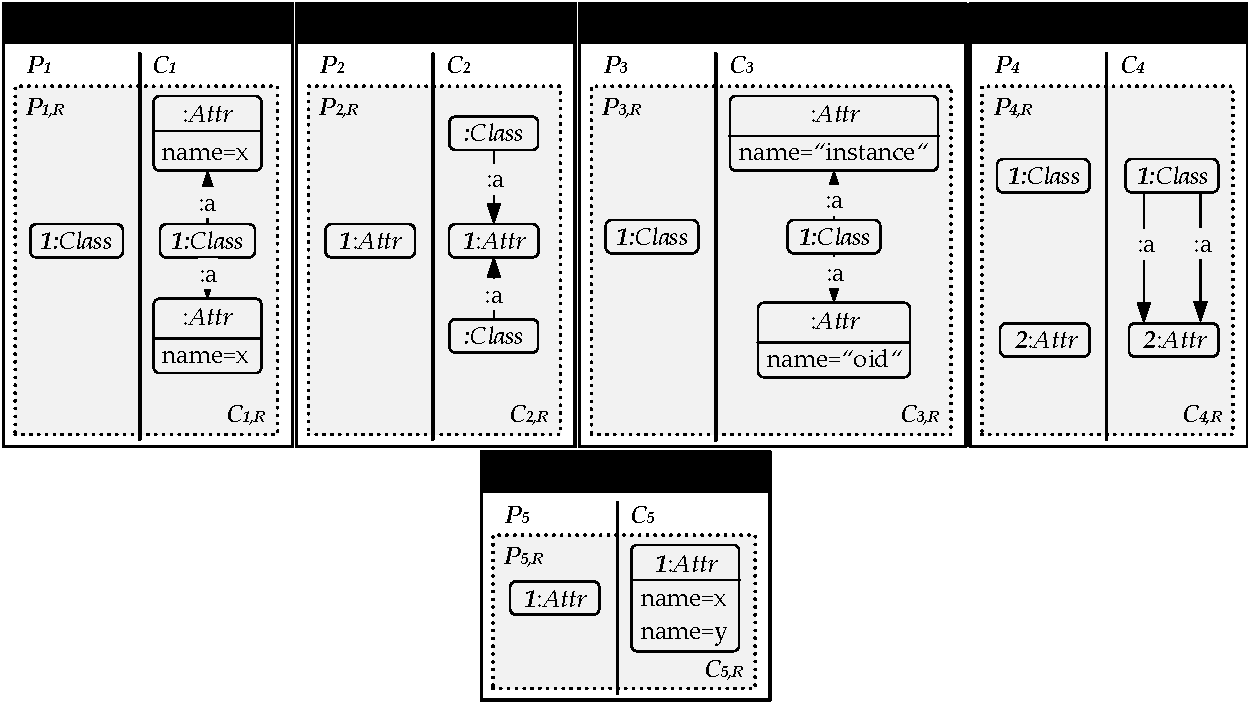
\includegraphics[width=\textwidth]{img/domain_mt/constraints.pdf}};
\fill (-5.65,3.85) node[inner sep=1pt] (B) {\footnotesize{\textcolor{white}{$c_9=\neg\exists(P_1 \to C_1,\true)$}}};
\fill (-2.2,3.85) node[inner sep=1pt] (C) {\footnotesize{\textcolor{white}{$c_{10}=\neg\exists(P_2 \to C_2,\true)$}}};
\fill (1.2,3.85) node[inner sep=1pt] (D) {\footnotesize{\textcolor{white}{$c_{11}=\neg\exists(P_3 \to C_3,\true)$}}};
\fill (5.75,3.85) node[inner sep=1pt] (E) {\footnotesize{\textcolor{white}{$c_{12}=\neg\exists(P_4 \to C_4,\true)$}}};
\fill (0,-1.45) node[inner sep=1pt] (F) {\footnotesize{\textcolor{white}{$c_{13}=\neg\exists(P_5 \to C_5,\true)$}}};
\end{tikzpicture}
\end{center}
\caption{Additional Domain Graph Constraints with Restrictions}
\label{fig:sec-dom-compl-mt:constraints}
\end{figure}

\begin{figure}[!tb]
\begin{center}
\begin{tikzpicture}[]
\fill (0,0) node[inner sep=1pt] (A) {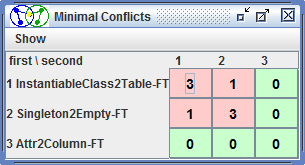
\includegraphics[width=.5\textwidth]{img/domain_mt/agg.png}};
\fill (-7.5,0) node[inner sep=1pt] (B) {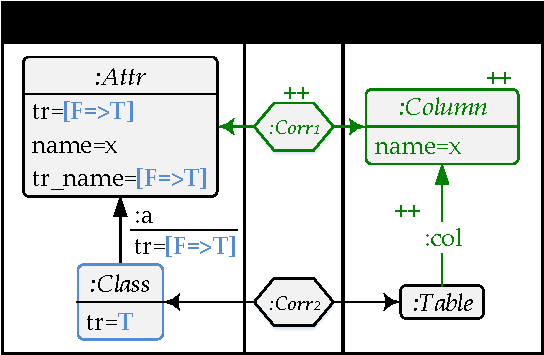
\includegraphics[width=.45\textwidth]{img/domain_mt/ft.pdf}};
\fill (-9.3,1.9) node[inner sep=1pt] (C) {\textcolor{white}{Attr2Column-FT}};
\end{tikzpicture}
\end{center}
\caption{Foward Translation Rule \code{Attr2Column-FT} (left) \& Conflict Analysis of Forward Translation Rules with AGG (right)}
\label{fig:sec-dom-compl-mt:agg}
\end{figure}

\begin{figure}[!tb]
\begin{center}
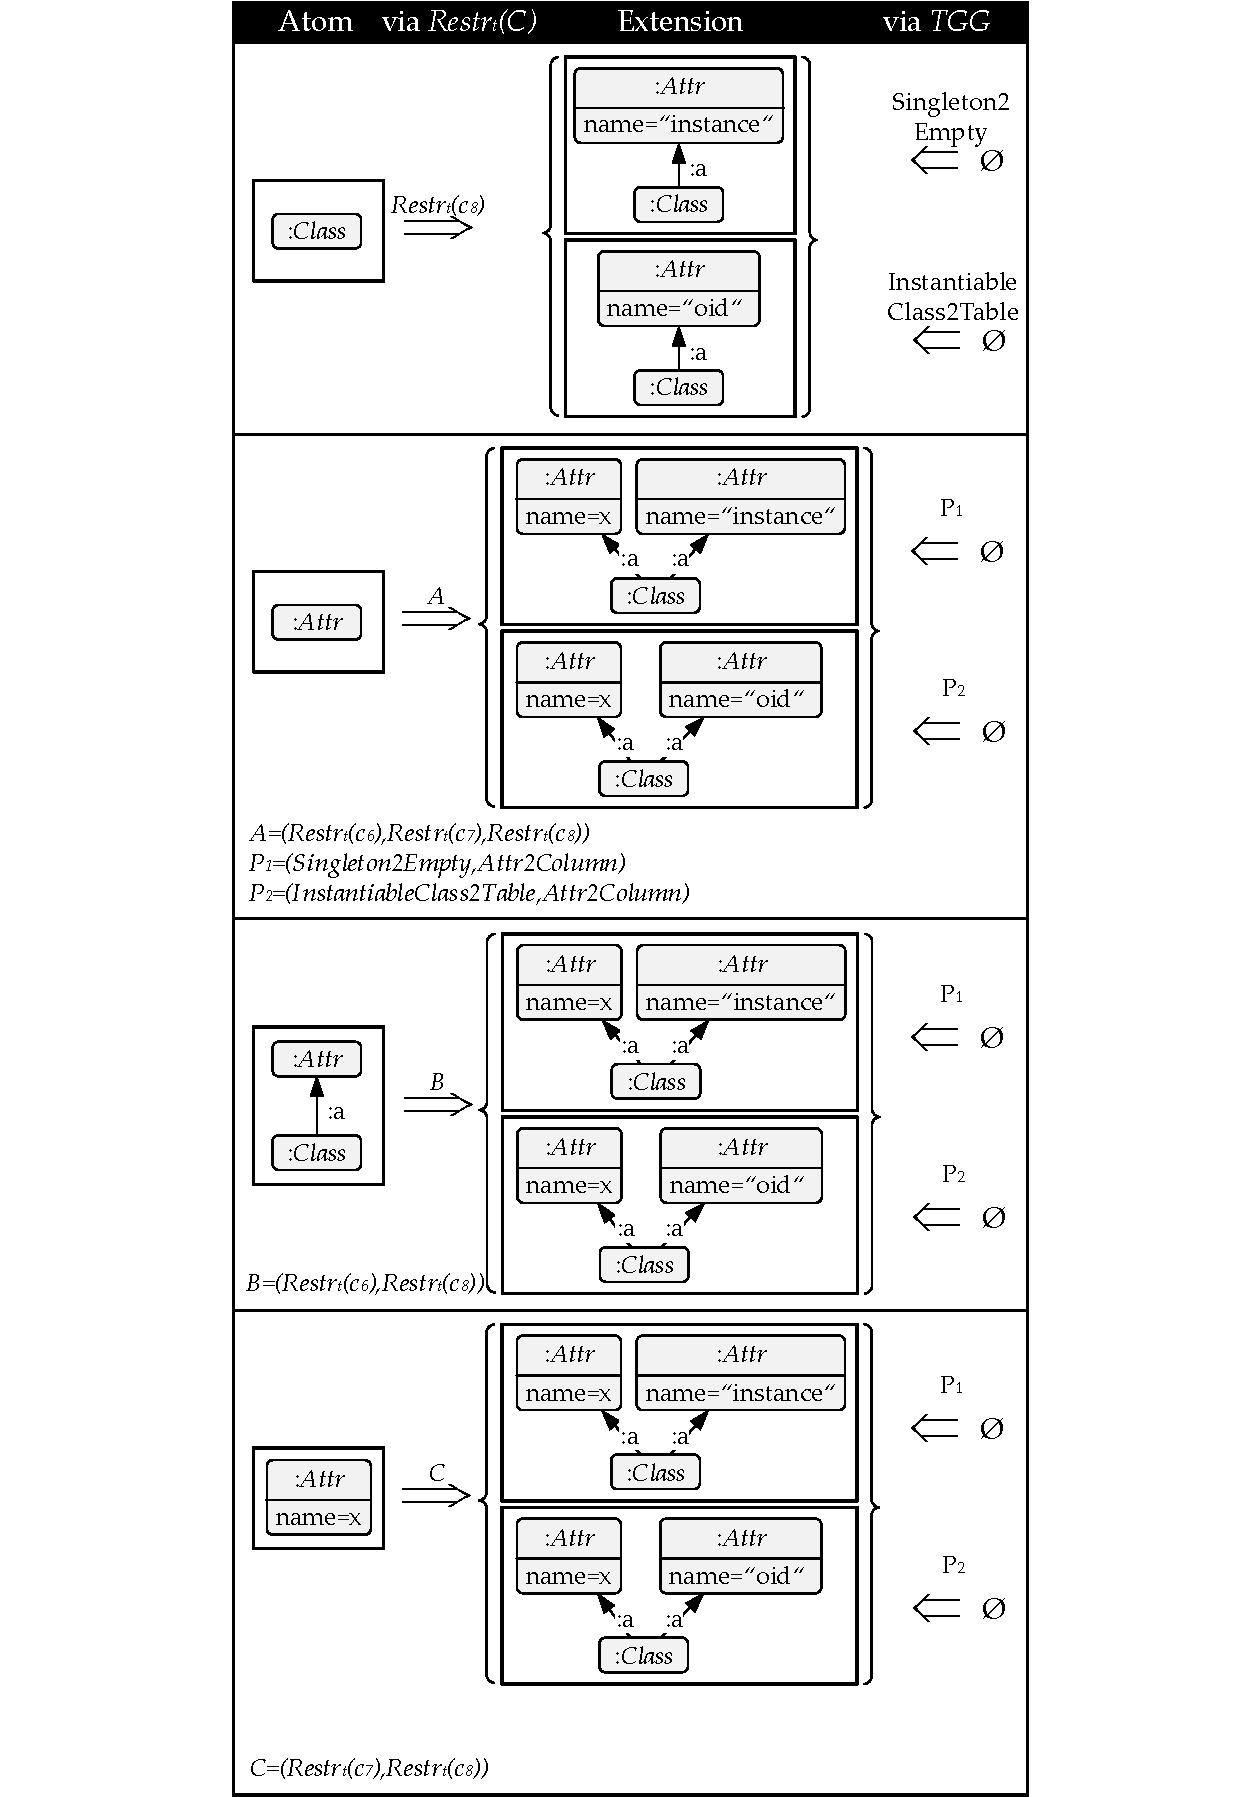
\includegraphics[width=\textwidth]{img/domain_mt/ext.pdf}
\end{center}
\caption{Verification of $\Restr_t(C)$-Extension Completeness of $\Lang(\TGG)^S$}
\label{fig:sec-dom-compl-mt:ext}
\end{figure}

\begin{example}[Domain Completeness of Model Transformations under Restrictions]
\label{fig:sec-dom-compl-mt:ex:dom_compl_1}
The model transformation $\MT\colon \Lang(C) \TransMT \Lang(\TG_\RDBM)$ from UML class diagrams (CDs) to relational database models (RDBMs) as defined by the $\TGG$ with empty start graph and triple rules without application conditions and typed over $\TG_{\CD,R}$ from \cref{sec-dc-general-res,fig:sec-dc-general:res_tg} is not domain complete w.r.t. the domain constraints $C=\{c_1,\ldots,c_{13}\}$ in \cref{fig:sec-dc-general:res_c,fig:sec-dc-general:res_ext,fig:sec-dom-compl-mt:constraints}, since, class constructors together with their visibilities are not covered by the given $\TGG$.
We assume that all constraints $c \in C$ are designated for general satisfaction, i.e., $C=C_I \cup C_G$ with $C_I=\varnothing$ and $C_G=C$.
However, the model transformation is domain complete under restrictions w.r.t. domain constraints $C$, the given $\TGG$, type morphism $t\colon \TG_{\CD,R} \to \TG_\CD \in \M$ and restriction $\TG_{\CD,R}$.
Thus, all \code{Class}es and \code{Attr}ibutes in each CD can be translated to corresponding \code{Table}s and \code{Column}s in RDBMs.
In order to show this, by \cref{thm:sec-dom-compl-mt:dom_compl_res_mt_II}, we have to verify domain completeness w.r.t. the restricted domain constraints $\Restr_t(C)$, the given $\TGG$ and restricted type graph $\TG_{\CD,R}$, i.e., by \cref{fact:sec-dom-compl-mt:comp} domain completeness of model transformation $\MT_R\colon \Lang(\Restr_t(C)) \TransMT \Lang(\TG_\RDBM)$ from class diagrams that are typed over $\TG_{\CD,R}$ and satisfy the restricted constraints $\Restr_t(C)$ to RDBMs that are typed over $\TG_\RDBM$.
By \cref{thm:sec-dom-compl-mt-without-acs}, we have to check that the forward translation rules of $\TGG$ are $\Restr_t(C)$-conflict-free and furthermore, $\Lang(\TGG)^S$ is $\Restr_t(C)$-extension complete.
According to \cref{sec-dc-general-res,thm:sec-dc-general-res:dom_compl_res}, $\Restr_t(C)=\{\Restr_t(c_1),\Restr_t(c_6),\Restr_t(c_7),\Restr_t(c_8),\Restr_t(c_9),\Restr_t(c_{10}),\Restr_t(c_{11}),\Restr_t(c_{12}),$ $\Restr_t(c_{13})\}$ while constraints $c_2$ to $c_5$ are neglected for the verification, as, they are positive but 
%not restricted 
unrestricted along $t$ ($c_2$ to $c_4$) or negative but not purely restricted along $t$ ($c_5$).
The restricted constraints are highlighted by grey boxes in \cref{fig:sec-dc-general:res_c,fig:sec-dc-general:res_ext,fig:sec-dom-compl-mt:constraints} with premises $P_{\_,R}$ and conclusions $C^{[E]}_{\_,R}$.
\cref{fig:sec-dom-compl-mt:agg} (left) shows the forward translation rule \code{Attr2Column-FT} of triple rule \code{Attr2Column} in \cref{fig:sec-dc-general:res_tg}.
Analogously, we derive forward translation rules \code{InstantiableClass2Table-FT} and \code{Singleton2Empty-FT} for triple rules \code{InstantiableClass2Table} and \code{Singleton2Empty}.
\cref{fig:sec-dom-compl-mt:agg} (right) depicts the result of the conflict analysis of the forward translation rules with AGG \cite{AGG} while omitting conflicts of the same rule and same match.
Altogether, there are eight conflicts that are reflected by constraints $c_9$ to $c_{12}$ in \cref{fig:sec-dom-compl-mt:constraints}, i.e., each conclusion represents a conflict graph where the conflict occurs in the premise part of the conclusion, respectively.
Note that the conflicts are actually caused by updates of translation attributes but the translation attributes are not depicted explicitly in \cref{fig:sec-dom-compl-mt:constraints}.
In more detail, between rule \code{InstantiableClass2Table-FT} itself and \code{Singleton2Empty-FT} itself there are three conflicts, respectively, as reflected by conclusions $C_1,C_2$ and $C_4$.
This is due to the fact that both rules may translate
\begin{enumerate*}
\item the same \code{Class} but not the same \code{Attr}ibute, or
\item the same attribute but not the same class, or
\item the same class and attribute but not the same edge \code{:a} the assigns the attribute to the class.
\end{enumerate*}
Therefore, we forbid the following obvious patterns in class diagrams by constraints $c_9,c_{10}$ and $c_{12}$:
\begin{enumerate*}
  \item Constraint $c_9$ claims that each class does not have two or more attributes of the same name.
  \item Constraint $c_{10}$ claims that each attribute is assigned to at most one class.
  \item Constraint $c_{12}$ claims that for each two classes and attributes there is at most one assignment edge \code{:a} between both.
\end{enumerate*}
Between rules \code{InstantiableClass2Table-FT} and \code{Singleton2Empty-FT} and vice versa there is one conflict, respectively, as reflected by conclusion $C_3$.
This is due to the fact that both rules may translate the same class while translating different attributes \code{``instance''} and \code{``oid''} of that class.
Therefore, we forbid the pattern of a class that has attributes \code{``instance''} and \code{``oid''} at the same time in class diagrams by constraint $c_{11}$, i.e., class diagrams are not allowed to contain classes that are both instantiable and singleton at the same time.
Thus, by adding constraints $c_9$ to $c_{12}$ to domain constraints $c_1$ to $c_8$, the forward translation rules are $\Restr_t(C)$-conflict-free.
It remains to verify that $\Lang(\TGG)^S$ is $\Restr_t(C)$-extension complete.
The successful verification is depicted in \cref{fig:sec-dom-compl-mt:ext}.
Each atom over restricted type graph $\TG_{\CD,R}$ can be extended via restricted constraints $\Restr_t(C)$ such that the extension can be created by applying the triple rules of the given $\TGG$ with starting at the empty start graph $\varnothing$:
\begin{enumerate}
  \item \label{fig:sec-dom-compl-mt:ex:item1} The atom with a single \code{:Class} node can be extended via $\Restr_t(c_8)$ to two graphs, i.e., one graph with additional \code{``instance''} attribute and one with additional \code{``oid''} attribute, and both graphs can be created via rule \code{Singleton2Empty} or \code{InstantiableClass2Table}, respectively.
  \item \label{fig:sec-dom-compl-mt:ex:item2} The atom with a single \code{:Attr}ibute node can be extended via restricted constraints $\Restr_t(c_6),\Restr_t(c_7)$ and $\Restr_t(c_8)$ successively to two graphs, i.e., one graph with two additional \code{``instance''} and \code{x} attributes and one with two additional \code{``oid''} and \code{x} attributes, and both graphs can be created via rules \code{Singleton2Empty} and \code{Attr2Column} OR \code{InstantiableClass2Table} and \code{Attr2Column} successively.
  \item \label{fig:sec-dom-compl-mt:ex:item3} The atom with an \code{:Attr}ibute node, \code{:Class} node and \code{:a}ssignment edge in between can be extended via $\Restr_t(c_6)$ and $\Restr_t(c_8)$ successively to the same two graphs as in \cref{fig:sec-dom-compl-mt:ex:item2}.
  \item \label{fig:sec-dom-compl-mt:ex:item4} The same is true for the atom with a single \code{:Attr}ibute node and node attribute \code{name} via $\Restr_t(c_7)$ and $\Restr_t(c_8)$ successively.
  Note that constraint $c_{13}$ is essential for building the extensions, e.g., the second extension step in \cref{fig:sec-dom-compl-mt:ex:item4} via $\Restr_t(c_8)$ may also lead to an overlapping resulting in an extension graph $G_E$ where node \code{:Attr} has two \code{name} attributes which cannot be created via the rules of the $\TGG$.
  However, due to constraint $c_{13}$, graph $G_E$ does not occur in extensions, since, $G_E$ is $\Restr_t(C)$-inconsistent according to \cref{def:C-extension}.
\end{enumerate}
Therefore, the model transformation $\MT_R$ from class diagrams typed over $\TG_{\CD,R}$ that satisfy the restricted domain constraints $\Restr_t(C)$ to RDBMs is domain complete implying further according to \cref{thm:sec-dom-compl-mt:dom_compl_res_mt_equiv} that the model transformation $\MT$ from class diagrams typed over $\TG_\CD$ that satisfy the original domain constraints $C$ to RDBMs is domain complete under restrictions w.r.t. the given $\TGG$, type morphism $t$ and restricted type graph $\TG_{\CD,R}$.
\envEndMarker
\end{example}

\begin{figure}[!tb]
\begin{center}
\begin{tikzpicture}[]
\fill (0,0) node[inner sep=1pt] (A) {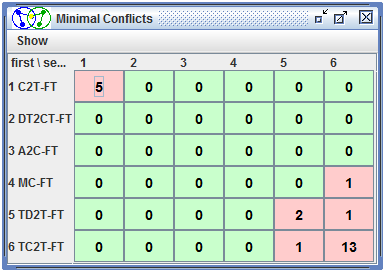
\includegraphics[width=.55\textwidth]{img/domain_mt/agg2.png}};
\fill (-7.75,0) node[inner sep=1pt] (B) {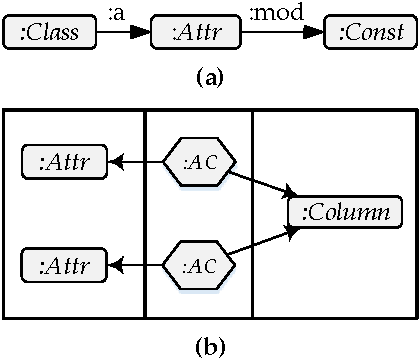
\includegraphics[width=.4\textwidth]{img/domain_mt/pattern.pdf}};
\end{tikzpicture}
\end{center}
\caption{Graph Pattern of Conflict Graphs (a) and (b) \& Conflict Analysis of Forward Translation Rules with AGG (right)}
\label{fig:sec-dom-compl-mt:agg2}
\end{figure}

\begin{example}[Domain Completeness of Model Transformations with Application Conditions]
\label{ex:sec-dom-compl-mt:domcp}
Given the model transformation CD2RDBM from UML class diagrams to relational database models in \cref{sec-mt-tgg,ex:sec-mt-tgg:fwd_mt} based on the forward translation rules $\TR_\FT$ of the triple rules $\TR$ with application conditions in \cref{sec-gt-trafo,fig:sec-gt-trafo:tgg} with triple graph grammar $CD2RDBM=(\varnothing,\TR)$ in \cref{sec-tgg,ex:sec-tgg:tg} that is typed over triple type graph $\TG=(\TG_\CD \gets \TG_C \to \TG_\RDBM)$ in \cref{sec-gt-graphs,fig:sec-gt-graphs:atg}.
Furthermore, given the source domain constraints $C^S$ for UML class diagrams in \cref{sec-gt-gc,ex:sec-gc-gc:gc_UML_CD} that are typed over type graph $\TG_\CD$.
\cref{fig:sec-dom-compl-mt:agg2} (right) depicts the result of the conflict analysis of forward translation rules $\TR_\FT$ via AGG \cite{AGG} where all critical pairs that are directly strict confluent and all critical pairs with conflict graphs that do not satisfy the multiplicity constraints in $\TG_\CD$ in the source component, respectively, are already omitted.
Note that critical pairs with conflict graphs whose source component violates a negative constraint in $C^S$ is $C^S$-inconsistent according to \cref{def:sec-dom-compl-mt:cf-fwd,def:sec-dom-compl-mt:cf-fwd:1} and therefore also not significant w.r.t. $\Lang(C^S)$ by \cref{sec-dc-verification,rem:sec-gc-verification} and thus, can be omitted by \cref{def:sec-dom-compl-mt:cf-fwd,def:sec-dom-compl-mt:cf-fwd:1}.
In total there are the following 23 critical pairs remaining:
\begin{enumerate}
  \item For forward translation rule \code{C2T-FT}, the source component of the conflict graph $O$ of each of the five critical pairs contains two \code{Classes} having the same \code{name} which is forbidden by constraint \code{12}.
  Therefore, the five critical pairs can be omitted by \cref{def:sec-dom-compl-mt:cf-fwd,def:sec-dom-compl-mt:cf-fwd:1}.
  \item For the critical pair of rules \code{MC-FT} and \code{TC2T-FT}, the source component of the conflict graph contains graph pattern \cref{fig:sec-dom-compl-mt:agg2} (a) which is forbidden by constraints \code{9} and \code{15}.
  Therefore, this critical pair can be omitted by \cref{def:sec-dom-compl-mt:cf-fwd,def:sec-dom-compl-mt:cf-fwd:1}.
  \item The conflict graphs of the remaining critical pairs contain triple graph pattern \cref{fig:sec-dom-compl-mt:agg2} (b), respectively, which cannot be created by forward translation sequences via $\TR_\FT$.
  Thus, these critical pairs can also be omitted by \cref{def:sec-dom-compl-mt:cf-fwd,def:sec-dom-compl-mt:cf-fwd:2}.
\end{enumerate}
Therefore, the forward translation rules $\TR_\FT$ are $C^S$-conflict-free.
$C^S$-extension completeness of $\Lang(CD2RDBM')^S$ can be successfully verified analogously to the verification of $C$-extension completeness in \cref{sec-dc-verification,ex:c-extension-compl} but this time without a projection to the source domain only. 
Therefore, $\Lang(C^S) \subseteq \Lang(CD2RDBM)^S$ by \cref{thm:sec-dom-compl-mt-without-acs}.
Thus, model transformation $CD2RDBM$ is domain complete by \cref{fact:sec-dom-compl-mt:comp}.
Therefore, all (infinitely many) UML class diagrams that satisfy the source domain constraints $C^S$ can be transformed to relational database models.
\envEndMarker
\end{example}